\chapterimage{potw1712a2}% Chapter heading image

%\chapter{Week7}

\section{Thursday}\index{week7_Thursday_lecture}

Three ways for matrix decomposition are significant in linear alegbra:
\[
\left\{
\begin{lgathered}
\text{LU (from \emph{elimination})}\\
\text{QR (from \emph{orthogonalization})}\\
\text{SVD (from \emph{eigenvectors})}
\end{lgathered}
\right.
\]
We have learnt the first two decomposition. And the third way is increasingly significant in the information age.\\
In the last lecture we talk about \textit{eigendecomposition} for \emph{real symmetric} matrices and \textit{diagonalization}. However, can we get some \emph{universal} decomposition? Is there any decomposition that can be applied to all matrices?\\
The anwer is yes. The key idea is to do \textit{symmetrization}, we have to consider $\bm A\bm A\trans$ and $\bm A\trans\bm A$.
\subsection{SVD: Singular Value Decomposition}
Any matrix $\bm A\in\mathbb{R}^{m\x n}$ could be factorized into
\[
\bm A=\bm U\bm\Sigma\bm V\trans
\]
where $\bm U$ is a $m\x m$ \emph{orthogonal} matrix,
$\bm\Sigma$ is a $m\x n$ ``\textit{diagonal}'' (we will define it later) matrix,
$\bm V$ is a $n\x n$ \emph{orthogonal} matrix.\\
If $\bm V$=$\bm U$ (then consequently $m=n$), then this is exactly \textit{eigendecomposition}.\\
Specifically speaking,\\
$\bm U$ is $m\x m$ matrix s.t. \textit{columns are eigenvectors of $\bm A\bm A\trans$.}\\
$\bm V$ is $n\x n$ matrix s.t. \textit{columns are eigenvectors of $\bm A\trans\bm A$.}\\
$\bm\Sigma$ is $m\x n$ matrix which has the form:
\[
\bm\Sigma=\begin{pmatrix}
\sigma_1&&\\&\ddots&\\&&\sigma_n\\
0&\dots&0\\\vdots&\ddots&\vdots\\0&\dots&0
\end{pmatrix}\text{ if $m\ge n$}\quad\text{or }
\bm\Sigma=\begin{pmatrix}
\sigma_1&&&0&\dots&0\\&\ddots&&\vdots&\ddots&\vdots\\&&\sigma_m&0&\dots&0\end{pmatrix}\text{ if $m< n$}.
\]
And $\sigma_i=\sqrt{\lambda_i}$ for $i=1,2,\dots,\min\{m,n\}$, where \textit{$\lambda_i$'s are eigenvalues of $\bm A\bm A\trans$ or $\bm A\trans\bm A$.} (if $m\ge n$), then $\lambda_i$'s are eigenvalues of $\bm A\trans\bm A$; otherwise $\lambda_i$'s are eigenvalues of $\bm A\bm A\trans$.)
\begin{theorem}
SVD always exists for any \emph{real} matrix.
\end{theorem}
\begin{proof}
For any $m\x n$ matrix $\bm A$, WLOG, we set $m\ge n$.
\begin{itemize}
\item
Firstly, we consider the case that all $\lambda_j\ne0$ for $j=1,\dots,n$. ($\lambda_j$'s are eigenvalues of $\bm A\trans\bm A$.)\\
Since $\bm A\trans\bm A$ is \textit{real symmetric}, we do the eigendecomposition:
\[
\bm A\trans\bm A=\bm V\bm D\bm V\trans
\]
where $\bm V$ is \textit{orthonormal} matrix and $\bm D$ is \textit{diagonal} matrix.\\
Also, the eigenvectors of $\bm A\trans\bm A$ are orthogonal (note that in proposition (16.3) we claim that the eigenvectors of diagonalizable matrix are orthogonal.):
\enlargethispage{1cm}
\[
\bm A\trans\bm A\bm v_j=\lambda_j\bm v_j\text{ for }j=1,\dots,n
\]
where $\bm v_j$'s are eigenvectors of $\bm A\trans\bm A$ s.t. they form orthonormal basis of $\mathbb{R}^n$.\\
\newpage
Note that given any matrix $\bm A$, $\bm V=\begin{bmatrix}
\bm v_1&\dots&\bm v_n
\end{bmatrix}$ is immediately defined. (This is because $\bm v_j$'s are eigenvectors of $\bm A\trans\bm A$.)\\
If we want to show $\bm A=\bm U\bm\Sigma\bm V\trans$, since $\bm A$ and $\bm V$ is defined, we only need to show there exists \textit{special} $\bm U$ and $\bm\Sigma$ such that
\[
\bm U\bm\Sigma=\bm A(\bm V\trans)^{-1}=\bm A\bm V.
\]
\begin{itemize}
\item
First step, we construct such $\bm U$ and $\bm\Sigma$:\\
Since $\lambda_j$'s are eigenvalues of $\bm A\trans\bm A$ associated with eigenvectors $\bm v_j$, we obtain:
\[
\|\bm A\bm v_j\|^2=\bm v_j\trans(\bm A\trans\bm A\bm v_j)=\bm v_j\trans(\lambda_j\bm v_j)=\lambda_j(\bm v_j\trans\bm v_j)=\lambda_j\|\bm v_j\|^2.
\]
Hence $\lambda_j=\frac{\|\bm A\bm v_j\|^2}{\|\bm v_j\|^2}>0$. (As we assume $\lambda_j\ne0$, this is strictly inequality.)\\
Hence we define $\bm u_j:=\bm A\bm v_j\frac{1}{\sqrt{\lambda_j}}\in\mathbb{R}^{m\x 1}.$ for $j=1,\dots,n$.\\
And then we construct $\bm U$ and $\bm\Sigma$:
\begin{align*}
\bm U:&=\begin{bmatrix}
\bm u_1&\dots&\bm u_n
\end{bmatrix}\in\mathbb{R}^{m\x n}.\\
\bm\Sigma:&=\diag(\sqrt{\lambda_1},\dots,\sqrt{\lambda_n})\in\mathbb{R}^{n\x n}.
\end{align*}
It's easy to verify that $\bm U\bm\Sigma=\bm{AV}$.
\item
Next step, we show that $\{\bm u_1,\dots,\bm u_n\}$ is orthonormal set:\\
For any $\bm u_i,\bm u_j$, we have
\begin{align*}
\inp{\bm u_i}{\bm u_j}&=\frac{1}{\sqrt{\lambda_i}\sqrt{\lambda_j}}\inp{\bm A\bm v_i}{\bm A\bm v_j}\\
&=\frac{1}{\sqrt{\lambda_i}\sqrt{\lambda_j}}\inp{\bm v_i}{\bm A\trans\bm A\bm v_j}
\qquad\text{Due to the useful formula $\inp{\bm{Ax}}{\bm y}=\inp{\bm x}{\bm A\Her\bm y}$.}
\\
&=\frac{1}{\sqrt{\lambda_i}\sqrt{\lambda_j}}\inp{\bm v_i}{\lambda_j\bm v_j}=
\sqrt{\frac{\lambda_j}{\lambda_i}}\inp{\bm v_i}{\bm v_j}
\end{align*}
Since $\{\bm v_1,\dots,\bm v_n\}$ are orthonormal, we obtain
\[
\inp{\bm v_i}{\bm v_j}=\begin{cases}
1,&i=j\\
0,&i\ne j
\end{cases}\implies
\inp{\bm u_i}{\bm u_j}=\begin{cases}
1,&i=j\\
0,&i\ne j
\end{cases}
\]
Hence $\{\bm u_1,\dots,\bm u_n\}$ are orthonormal.
\item
Then we show that $\{\bm u_1,\dots,\bm u_n\}$ are eigenvectors of $\bm A\bm A\trans$:\\
For $j=1,\dots,n$, we obtain:
\begin{align*}
\bm A\bm A\trans\bm u_j&=\bm A\bm A\trans\bm A\bm v_j\frac{1}{\sqrt{\lambda_j}}\qquad\text{by definition of $\bm u_j$.}\\
&=\bm A(\bm A\trans\bm A\bm v_j)\frac{1}{\sqrt{\lambda_j}}=\bm A\lambda_j\bm v_j\frac{1}{\sqrt{\lambda_j}}\\
&=\sqrt{\lambda_j}\bm A\bm v_j=\lambda_j\times(\frac{1}{\sqrt{\lambda_j}}\bm A\bm v_j)\\
&=\lambda_j\bm u_j.
\end{align*}
\item
We notice that in SVD $\bm U$ is m by m matrix, $\bm\Sigma$ is m by n matrix. Hence we need to \textit{reconstruct} our $\bm U$ and $\bm\Sigma$ in step 1:\\
Since $\{\bm u_1,\dots,\bm u_n\}$ are eigenvectors of $\bm A\bm A\trans$, and $\bm A\bm A\trans$ has $m$ orthogonal eigenvectors, so we pick $\bm u_{n+1},\dots,\bm u_m$ s.t. $\{\bm u_1,\dots,\bm u_{n},\bm u_{n+1},\dots,\bm u_m\}$ are $m$ orthonormal eigenvectors of $\bm A\bm A\trans$.\\
Then we let
\begin{gather*}
\bm U:=\begin{bmatrix}
\bm u_1&\dots&\bm u_m
\end{bmatrix}\in\mathbb{R}^{m\x m}.\\
\bm\Sigma:=\begin{pmatrix}
\sqrt{\lambda_1}&&\\&\ddots&\\&&\sqrt{\lambda_n}\\
0&\dots&0\\\vdots&\ddots&\vdots\\0&\dots&0
\end{pmatrix}\in\mathbb{R}^{m\x n}.
\end{gather*}
It's easy to verify that 
\[
\bm U\bm\Sigma=\bm{AV}
\]
Hence finally we obtain
\[
\bm U\bm\Sigma\bm V\trans=\bm A\bm V\bm V\trans=\bm A.
\]
\end{itemize}
\item
For there exists some $\lambda_j=0$ case, we discuss it in next section.
\end{itemize}
\end{proof}
\subsection{Remark on SVD decomposition}
\subsubsection{Remark 1}
The eigenvalues for $\bm A\trans\bm A$ and $\bm A\bm A\trans$ are not always nonzero.
\begin{proposition}
For $m\x n$ matrix $\bm A$, suppose $\rank(\bm A)=r$,
and the eigenvalues for $\bm A\trans\bm A$ are 
\[
\eig(\bm A\trans\bm A)=\{\lambda_1,\dots,\lambda_r,\overbrace{0,\dots\dots,0}^{\text{Totally $n-r$ terms}}\}, 
\]
then eigenvalues for $\bm A\bm A\trans$ are
\[
\eig(\bm A\bm A\trans)=\{\lambda_1,\dots,\lambda_r,\underbrace{0,\dots\dots,0}_{\text{Totally $m-r$ terms}}\}.
\]
\end{proposition}
\begin{proof}
\begin{itemize}
\item
Firstly let's prove a lemma:
\[
\det(\bm I_m-\bm{AB})=\det(\bm I_n-\bm{BA}).,
\]
where $\bm A\in\mathbb{R}^{m\x n}$ and $\bm B\in\mathbb{R}^{n\x m}.$\\
We notice the two equality:
\begin{align}
\begin{pmatrix}
\bm I_n&\bm B\\
\bm A&\bm I_m
\end{pmatrix}\begin{pmatrix}
\bm I_n&-\bm B\\
\bm 0_{m\x n}&\bm I_m
\end{pmatrix}
&=\begin{pmatrix}
\bm I_n&\bm 0_{n\x m}\\
\bm A&\bm I_m-\bm{AB}
\end{pmatrix}\\
\begin{pmatrix}
\bm I_n&-\bm B\\
\bm 0_{m\x n}&\bm I_m
\end{pmatrix}
\begin{pmatrix}
\bm I_n&\bm B\\
\bm A&\bm I_m
\end{pmatrix}
&=\begin{pmatrix}
\bm I_n-\bm{BA}&\bm 0_{n\x m}\\
\bm A&\bm I_m
\end{pmatrix}
\end{align}
We take determinant both sides for the two equations above:
\begin{align}
\begin{vmatrix}
\bm I_n&\bm B\\
\bm A&\bm I_m
\end{vmatrix}\begin{vmatrix}
\bm I_n&-\bm B\\
\bm 0_{m\x n}&\bm I_m
\end{vmatrix}
&=\begin{vmatrix}
\bm I_n&\bm 0_{n\x m}\\
\bm A&\bm I_m-\bm{AB}
\end{vmatrix}\\
\begin{vmatrix}
\bm I_n&-\bm B\\
\bm 0_{m\x n}&\bm I_m
\end{vmatrix}
\begin{vmatrix}
\bm I_n&\bm B\\
\bm A&\bm I_m
\end{vmatrix}
&=\begin{vmatrix}
\bm I_n-\bm{BA}&\bm 0_{n\x m}\\
\bm A&\bm I_m
\end{vmatrix}
\end{align}
Since we have $\begin{vmatrix}
\bm I_n&\bm B\\
\bm A&\bm I_m
\end{vmatrix}\begin{vmatrix}
\bm I_n&-\bm B\\
\bm 0_{m\x n}&\bm I_m
\end{vmatrix}=\begin{vmatrix}
\bm I_n&-\bm B\\
\bm 0_{m\x n}&\bm I_m
\end{vmatrix}
\begin{vmatrix}
\bm I_n&\bm B\\
\bm A&\bm I_m
\end{vmatrix},$ we derive
\[
\begin{vmatrix}
\bm I_n&\bm 0_{n\x m}\\
\bm A&\bm I_m-\bm{AB}
\end{vmatrix}=\begin{vmatrix}
\bm I_n-\bm{BA}&\bm 0_{n\x m}\\
\bm A&\bm I_m
\end{vmatrix}
\implies
\det(\bm I_n)\det(\bm I_m-\bm{AB})=\det(\bm I_m)\det(\bm I_n-\bm{BA})
\]
Equivalently, $\det(\bm I_m-\bm{AB})=\det(\bm I_n-\bm{BA}).$
\item
Secondly we prove that the nonzero eigenvalues of $\bm A\trans\bm A$ and $\bm A\bm A\trans$ are exactly the same (counted with multiplicity):\\
We only need to show $\frac{\det(\lambda\bm I-\bm A\trans\bm A)}{\lambda^{n-r}}=\frac{\det(\lambda\bm I-\bm A\trans\bm A)}{\lambda^{m-r}}.$\\
And we find that 
\begin{align*}
\det(\lambda\bm I-\bm A\trans\bm A)&
=\lambda^n\det(\bm I-\lambda^{-1}\bm A\trans\bm A)\\
&=\lambda^n\det(\bm I-\lambda^{-1}\bm A\bm A\trans)\qquad&\text{Due to Sylvester's determinant identity}\\
&&\text{$\det(\bm I_m-\bm{AB})=\det(\bm I_n-\bm{BA}).$}\\
&&\text{for $\bm A\in\mathbb{R}^{m\x n}$ and $\bm B\in\mathbb{R}^{n\x m}$.}
\end{align*}
Hence we obtain
\begin{align*}
\frac{\det(\lambda\bm I-\bm A\trans\bm A)}{\lambda^{n-r}}&=\frac{\lambda^n\det(\bm I-\lambda^{-1}\bm A\bm A\trans)}{\lambda^{n-r}}\\
&=\frac{\lambda^m\det(\bm I-\lambda^{-1}\bm A\bm A\trans)}{\lambda^{m-r}}\\
&=\frac{\det(\lambda\bm I-\bm A\bm A\trans)}{\lambda^{m-r}}
\end{align*}
\item
Then we show the eigenvalues for $\bm A\trans\bm A$ have exactly $(n-r)$ zeros; the eigenvalues for $\bm A\bm A\trans$ have exactly $(m-r)$ zeros.\\
Assume there are $n$ ind. eigenvectors $\{\bm v_1,\dots,\bm v_n\}$ for $\bm A\trans\bm A$ corresponding to their eigenvalues $\{\lambda_1,\lambda_2,\dots,\lambda_n\}$. Hence we have
\[
\bm A\trans\bm A\bm v_i=\lambda_i\bm v_i\text{ for }i=1,\dots,n.
\]
Since $\rank(\bm A)=r=\rank(\bm A\trans\bm A)$, the dimension of the eigenspace for $\lambda=0$ is $n-r$.\\
Hence among $\{\bm v_1,\dots,\bm v_n\}$ there are $n-r$ ind. eigenvectors belong to the eigenspace for $\lambda=0$.\\
Thus there are exactly $(n-r)$ zeros for eigenvalues of $\bm A\trans\bm A$.
\item
How to prove there are exactly $(m-r)$ zeros for eigenvalues of $\bm A\bm A\trans$? We just need to obtain $\rank(\bm A\trans)=r=\rank(\bm A\bm A\trans)$ and proceed similarly.
\end{itemize}
\end{proof}
\newpage
\begin{remark}
Maybe you think the second part proof ($\bm A\trans\bm A$ and $\bm A\bm A\trans$ have the same set of nonzero eigenvalues) is too thicky. Here is a proofoutline of another way to show this conclusion:
\begin{proof}[Proofoutline.]\qquad\\
Assume $\bm v_1,\dots,\bm v_n$'s are eigenvectors of $\bm A\trans\bm A$, then define $\bm u_j$ as in the proof of SVD theorem for nonzero $\lambda_j$'s, where $j=1,\dots,r.$ \\
Then by the equation $\bm A\bm A\trans\bm u_j = \lambda_j\bm u_j$, $\lambda_j$ is also the eigenvalue of $\bm A\bm A\trans$ with eigenvector $\bm u_j$. 
\begin{itemize}
\item
If $\lambda_j$ is eigenvalue of $\bm A\trans\bm A$ with mulplicity $d$, then by the eigendecomposition there are exactly $d$ ind. eigenvectors $v_{j_1},\dots, v_{j_d}$ associated with $\lambda_j$; thus we get d ind. eigenvectors $\bm u_{j_1},\dots, \bm u_{j_d}$ associated with $\lambda_j$ for $\bm A\bm A\trans$. Thus the multiplicity of $\lambda_j$ for $\bm A\trans \bm A$ and $\bm A\bm A\trans$ are the same.
\item
Thus $\{\lambda_1, \dots, \lambda_r\}$ (counted with multiplicity) is a subset of $\eig(\bm A\bm A\trans)$.
\item
Similarly, the set of nonzero eigenvalues of $\bm A\bm A\trans$ is also a subset of $\eig(\bm A\trans\bm A)$. Thus these two matrices have the same set of nonzero eigenvalues.
\end{itemize}
   Since all the rest eigenvalues must be zero, we get the desired result. 
\end{proof}
\end{remark}

For SVD decomposition
\[
\bm A=\bm U\bm\Sigma\bm V\trans
\]
we can convert it into the following two forms:
\begin{gather*}
\bm A\bm V=\bm U\bm\Sigma\bm V\trans\bm V=\bm U\bm\Sigma\\
\bm A=\bm U\bm\Sigma\bm V\trans\implies
\bm A\trans=\bm V\bm\Sigma\bm U\trans\implies
\bm A\trans\bm U=\bm V\bm\Sigma\bm U\trans\bm U=\bm V\bm\Sigma.
\end{gather*}
If we write it into vector forms, we obtain:
\[
\left\{
\begin{aligned}
\bm A\bm v_j=\sigma_j\bm u_j\\
\bm A\trans\bm u_j=\sigma_j\bm v_j
\end{aligned}
\right.
\]
And the columns of $\bm U$ ($\bm u_j$) are called \emph{left singular vector} of $\bm A$; the columns of $\bm V$ ($\bm v_j$) are called \emph{right singular vector} of $\bm A$; $\sigma_j$ is called the \emph{singular value}.
\subsubsection{Remark 2: Four fundamental subspaces}
The general SVD decomposition for $\bm A\in\mathbb{R}^{m\x n}$ is given by
\[
\bm A=\begin{bmatrix}
\bm u_1&\dots&\bm u_r&\dots&\bm u_m
\end{bmatrix}\begin{pmatrix}
\sigma_1&&&&&\\
&\ddots&&&&\\
&&\sigma_r&&&\\
&&&0&&\\
&&&&\ddots&\\
&&&&&0\\
0&\dots&\dots&\dots&\dots&0\\
0&\dots&\dots&\dots&\dots&0\\
\end{pmatrix}
\begin{pmatrix}
\bm v_1\trans\\\vdots\\\bm v_r\trans\\\vdots\\\bm v_n\trans
\end{pmatrix}=\bm U\bm\Sigma\bm V\trans
\]
For such $\bm A$, the matrix $\bm U$ and $\bm V$ contain orthonormal basis for all four fundamental subspaces:
\begin{align*}
&\text{First }r\text{ columns of $\bm V$: }\text{row space of $\bm A$.}\\
&\text{last }n-r\text{ columns of $\bm V$: }\text{null space of $\bm A$.}\\
&\text{First }r\text{ columns of $\bm U$: }\text{column space of $\bm A$.}\\
&\text{last }m-r\text{ columns of $\bm U$: }\text{null space of $\bm A\trans$.}\\
\end{align*}
Maybe it's easy to understand it in graph:
\begin{figure}[H]
\centering
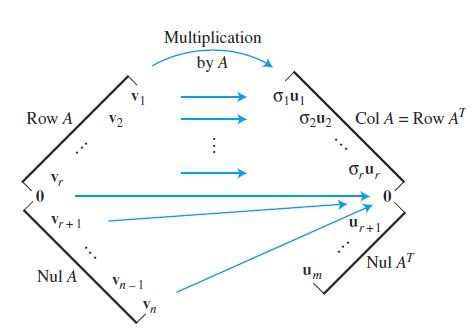
\includegraphics[width=10cm]{week7/fundamental}
\caption{The fundamental spaces and the action of $\bm A$.}
\end{figure}
\subsubsection{Remark 3: vector form}
Recall we can write eigendecomposition in \textit{vector form:}
\[
\bm A=\lambda_1\bm v_1\bm v_1\trans+\dots+\lambda_n\bm v_n\bm v_n\trans
\]
Also, we could write the \emph{general} SVD decomposition in remark 2 into \textit{vector form}:
\[
\bm A=\sigma\bm u_1\bm v_1\trans+\dots+\sigma\bm u_r\bm v_r\trans
\]
where $r=\rank(\bm A)=\text{number of nonzero singular values.}$ Here leads to the third meaning for the rank:
\begin{proposition}
The rank of $m\x n$ matrix $\bm A$ is the number of nonzero singular values.
\end{proposition}
\begin{proof}
Without loss of generality, we set $m\ge n$. And we assume there are exactly $s$ zero singular values of $\bm A$, which means there are $s$ zero eigenvalues of $\bm A\trans\bm A$ assocaiated with their $s$ ind. eigenvectors. (Independence is due to the diagonalizable of $\bm A\trans\bm A$.) In other words, the eigenspace of $\bm A\trans\bm A$ for $\lambda=0$ has dimension $s$.\\
The eigenspace of $\bm A\trans\bm A$ for $\lambda=0$ is given by
\[
\{\bm x:\bm A\trans\bm A\bm x=\bm 0\}.
\]
Hence its dimension is given by
\[
\rank(\bm A\trans\bm A)=\rank(\bm A):=n-r.
\]
Hence $s=n-r$. And obviously, the number of \emph{nonzero} singular values is $n-s=r$.
\end{proof}
\begin{remark}
However, $\rank(\bm A)\ne$ number of nonzero eigenvalues. Let me raise a counterexample:
\[
\bm A=\begin{bmatrix}
0&1\\0&0
\end{bmatrix}
\]
then eigenvalues are $\lambda_1=\lambda_2=0$, and $\rank(\bm A)=1.$
\end{remark}
\subsubsection{Compact SVD}
Hence any matrix with rank $r$ can be factorized into
\begin{align*}
\bm A&=\bm U\bm\Sigma\bm V\trans\\
&=\begin{bmatrix}
\bm u_1&\dots&\bm u_r
\end{bmatrix}\begin{pmatrix}
\sigma_1&&\\&\ddots&\\&&\sigma_r
\end{pmatrix}\begin{bmatrix}
\bm v_1\trans\\\vdots\\\bm v_r\trans
\end{bmatrix}
\end{align*}
where $\bm U\in\mathbb{R}^{m\x r}$ and $\bm V\in\mathbb{R}^{r\x n}$ are both orthogonal matrix. And $\bm\Sigma=\diag(\sigma_1,\dots,\sigma_r)$, where $\sigma_i>0$ for $i=1,2,\dots,r$.
\begin{corollary}
Every rank $r$ matrix can be written as the sum of $r$ rank $1$ matrices. Moreover, these matrices could be perpendicular!
\end{corollary}
What's the meaning of perpendicular?
\begin{definition}[perpendicular for matrix]
For two real $n\x n$ matrix $\bm A$ and $\bm B$, they are said to be \emph{perpendicular} (\emph{orthogonal}) if the inner product between $\bm A$ and $\bm B$ is zero:
\[
\inp{\bm A}{\bm B}=\trace(\bm B\trans\bm A)=\sum_{i,j=1}^{n}\bm A_{ij}B_{ij}=0.
\]
\end{definition}
Decompose $\bm A:=\sum_{i=1}^{r}\sigma_i\bm u_i\bm v_i\trans$. If we set $\bm A_i=\bm u_i\bm v_i\trans\sigma_i$, let's show $\bm A_i$'s are perpendicular:
\begin{align*}
\inp{\bm A_i}{\bm A_j}&=\trace(\bm A_j\trans\bm A_i)\\
&=\trace(\sigma_i\sigma_j\bm v_j\bm u_j\trans\bm u_i\bm v_i\trans)=\sigma_i\sigma_j\trace(\bm v_j\bm u_j\trans\bm u_i\bm v_i\trans)\\
&=\sigma_i\sigma_j\trace(\bm v_j(\bm u_j\trans\bm u_i)\bm v_i\trans)=\sigma_i\sigma_j\trace(\bm v_j\bm 0\bm v_i\trans)\\
&=0.
\end{align*}
So what is rank? How many rank 1 matrices do we need to pick to construct matrix $\bm A$? In fact, this number has no upper bound. For example, if we obtain
\[
\bm A=\bm u_1\bm v_1\trans+\bm u_2\bm v_2\trans
\]
Then we can always decompose any rank 1 matrix into 2 rank 1 matrix:
\[
\bm A=\bm u_1\bm v_1\trans+\frac{1}{2}\bm u_2\bm v_2\trans+\frac{1}{2}\bm u_2\bm v_2\trans.
\]
But this number has a lower bound, that is rank. In other words, $\rank(\bm A)$=smallest number of rank 1 matrices with sum $\bm A$.
\begin{remark}
Up till now, $\rank(\bm A)$ has three meanings:
\begin{itemize}
\item
$\rank(\bm A)=\dim(\row(\bm A))$
\item
$\rank(\bm A)=\dim(\col(\bm A))$
\item
$\rank(\bm A)=$ smallest number of rank 1 matrices with sum $\bm A$.
\end{itemize}
\end{remark}
\subsection{Best Low-Rank Approximation}
Given matrix $\bm A$. What is the \textit{best rank $k$ approximation}? In other words, given matrix $\bm A\in\mathbb{R}^{m\x n}$, what is the optimal solution for the model:
\begin{align*}
  \min\quad        & \|\bm A-\bm Z\|^2_{F} \\
  \text{s.t.\quad} &  \rank(\bm Z)=k &     \\
                   &\bm Z\in\mathbb{R}^{m\x n}
\end{align*}
Firstly let's introduce the definition for Frobenius norm:
\begin{definition}[Frobenius norm]
The Frobenius norm for $m\x n$ matrix $\bm A$ is given by
\[
\|\bm A\|_{F}=\sqrt{\inp{\bm A}{\bm A}}=\sqrt{\trace(\bm A\trans\bm A)}.
\]
\end{definition}
\begin{theorem}\label{proposition_8.4}
Suppose the SVD if $\bm A\in\mathbb{R}^{m\x n}$ is given by
\[
\bm A=\sigma_1\bm u_1\bm v_1\trans+\dots+\sigma_r\bm u_r\bm v_r\trans.
\]
where $\bm u_i$'s and $\bm v_i$'s are $\mathbb{R}^{n}$ vectors. And we suppose $\sigma_1\ge\sigma_2\ge\dots\ge0$.\\
Then the best rank $k$($k\le r$) approximation of $\bm A$ is
\[
\bm A_k=\sigma_1\bm u_1\bm v_1\trans+\dots+\sigma_k\bm u_k\bm v_k\trans.
\]
\end{theorem}
For example, $\sigma_1\bm u_1\bm v_1\trans$ is the best rank 1 approximation.
\subsubsection{Analogy with least square problem}
For least square problem, the key is to do approximation for $\bm b\in\mathbb{R}^m$. In other words, we just do a projection from $\bm b$ to the plane $\{\bm{Ax}|\bm x\in\mathbb{R}^n\}$:
\begin{figure}[H]
\centering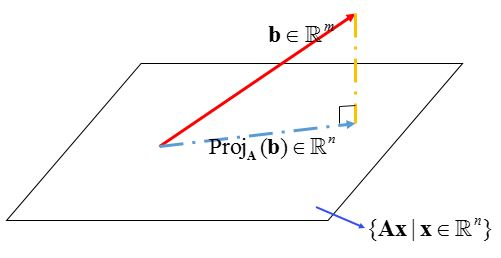
\includegraphics{week7/least_square}
\caption{Least square problem: find $\bm x$ such that $\bm{Ax}=\Proj_{\bm A}(\bm b).$}
\end{figure}
Similarly, the beast rank k approximation could be viewed as a projction from $\bm A$ with rank $r$ to the ``plane'' that contains all rank $k$ matrices:
\begin{figure}[H]
\centering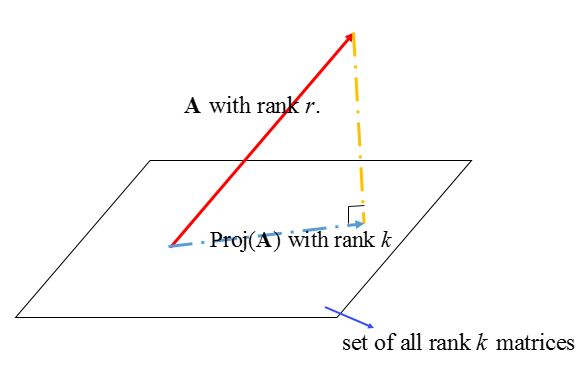
\includegraphics{week7/rank_r}
\caption{Best rank $k$ approximation: find projection from rank $r$ matrix to the plane that contains all rank $k$ matrices}
\end{figure}